\section{Conceptual Idea}

Haikunet is a SDN programming langauge which was created with the main objective of fulfilling the need of debugging the network, and creating an intent's oriented programming language agnostic to the controller. This last property means that Haikunet will not be coupled to a particular controller at all. Right now OpenDayLight and ONOS are the Controller's supported, but as you will see in following sections, enlarge this number is not hard at all, and you will have the chance to do this by following the tutorial.\\
Writing programs in Haikunet is really easy and straightforward, and this language will give you the advantage of having just one intent written in a common way for several controllers, something that up to now you weren't able to do as far as the writers of this thesis know.\\
The language is interpretated, written in Ruby and can be ran in any machine with a Ruby major or equal version of 2.0.0. This is how a program written in Haikunet looks like:

\begin{lstlisting}[language=Ruby,breaklines=true]
one_host := Host(mac="9A:4A:43:D4:36:45", vlan="-1", ipAddresses=["10.0.0.1"], elementId="of:0000000000000002", port="4")

second_host := Host(mac="72:D2:0D:24:C5:36", vlan="-1", ipAddresses=["10.0.0.4"], elementId="of:0000000000000003", port="4")

my_flow := Flow (src=one_host, dst=second_host, priority="55")

Intent firstExample
	Select my_flow
\end{lstlisting}

This program describes an intent for creating a flow between two host. We will come back to explain in more detailed this program and all the elements involve in the \textbf{Learning Haikunet} section.\\

The main ideas that you have to understand before writing a program in this language are the followings:

\begin{itemize}
\item Initial Topology\\
Which would be the initial topology?, think of this as the network in which you want to apply the intent. It's called initial because it can be seen as the initial point from where we start, and after the intent is applied to the newtork, we will obtain the desired network, which can be called the last one. In the \textbf{Formal Definition} section this is better explained.
\item What is what you want from the newtork?\\
Try to understand well what are you going to ask to the network, if it's possible to do it, which components are going to be involved in, etc. From this though, you will write your program.
\item Which is going to be the destiny?\\
Has the destiny the ability to do what you are expecting from the network?. Remember that you can always debug first what you are doing, and then proceed to apply it to the real network!.
\end{itemize}

After this, as every programming language, you will need to practice in order to write good programs. Let's take a look at the architectural components of the language, and how they relate one with each other.

\begin{figure}[H]
\centering
\includegraphics[width=\textwidth]{images/haikunet/arquitectura_haikunet.png}
\caption{Haikunet architectural view}
\end{figure}

The components in the left are the arguments the interpreter expect (except the topologygenerator tool which is a gem used by the language). We will come back in more detailed to these arguments in the \textbf{Learning Haikunet} section.\\
Inside the black box are the components which make up the interpreter, these will be explained in more detailed at the \textbf{Implementation} section, and finally at the right are the possible outputs that the language can provide (ONOS and OpenDayLight component's represent a generation of a bunch of request to one of these controllers, DEVS is the generation of the .pdm file, and finally ERROR represents that something went wrong while interpretating the program). These will also be seen in the \textbf{Learning Haikunet} section.\\

As it can be apreciated in the image, Haikunet uses the topologygenerator tool which was explained in the previous chapter. The topologygenerator gives an important characteristic to the language, which is that it allows us to create a NTM model and use it as our intial network, meaning that it's not mandatory to have a real network for using Haikunet. Another important thing is one of the destinies which Haikunet support's, DEVS. Supporting this destiny gives the language an important characteristic, which is permiting to simulate from either a real network or a NTM model how would an intent react in the initial newtork.\\

Haikunet flow's work as follow: We first run the interpreter giving as argument a progam and an output destiny, this output destiny specifies to which controller the program is being interpretated. The interpreter lexer's then receive the program, which will be in charge of tokenize it and give it to the parser, which will detect if the tokens are gramatically well written. After this, the semantic checker will detect either statical or dynamical errors in the program (we will explain in more detailed this erros definition's in the \textbf{Formal Definition} section), using the underlaying network which was given by the topologygenerator tool. After this two things can happen: either the program had no errors, meaning that the code generator will execute the bunch of request that have to be done to the API of the controllers specified in the input of the interpreter, or it had, this will cause an error raise exception with a message which will explain the problem. \\

This short paragraph resumes the working flow of a program being interprated by Haikunet. In the \textbf{Language Implementation} section we will cover in detailed what happens in each of the components previously mentioned.\\

Now that we have a better idea of what Haikunet is, let's proceed to give some formal definition's before getting into the tutorial, but before this let us explain you something.

\section{Why Haikunet?}

The name Haikunet comes from the join of Haiku and Network. A Haiku is a Japanese poem with a lot of themes, but in most of the cases a Haiku describes the nature from the view of an observer. This is exactly what you are going to do with Haikunet, write short programs which will describe the desired nature of a network, and this description will be done from the point of view of an observer of the network, meaning a person which does not necessarily knows how to interact at a system level with it, and in most of the cases, doesn't know how to. This is the intent's programmer point of view of the network. 

\section{Formal Definition}

In this section we will establish key concepts and main ideas that will be use in this chapter. The section will be divided in one definition after another, and after all definitions are made, we will continue with the Haikunet tutorial.\\

\subsection{Debugging}

Debugging will be the process of finding either static or dynamic errors before the intent is applied to the network. The definition of these type of erros can be found ahead in the section.\\
In this work, we are not going to explore techniques which involves stopping an intent execution's in a controller. 

\subsection{Error}

An error will be a request made by a program written in Haikunet, which has not semantically sense in the context of the current network. Since this definition involves a huge amount of errors for a thesis work, we will focus in a limited scope which will be introduced next. We will show some scenarios, their respectively errors in them, and the error output that the interpreter will show:

\subsubsection{Flow property definition error}

\textbf{Description:} This error happens when you use a host property in a flow definition, and this property cannot be neither found or inferred from the initial network topology. \\

\textbf{Example:} Let's suppose that we have the following initial network:

\begin{figure}[H]
\centering
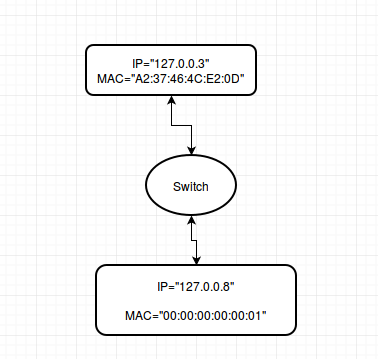
\includegraphics[width=\textwidth]{images/haikunet/error_scenario_1.png}
\caption{Initial network context in flow property definition error}
\end{figure}

and we execute the following program:

\begin{lstlisting}[language=Ruby,breaklines=true]
source_host := Host(mac="A2:37:46:4C:E2:0D")

my_flow := Flow (src=source_host, dst="127.0.0.10", priority="55")

Intent firstExample
    Select my_flow
\end{lstlisting}

In this example, we have the problem that the property \textit{dst = "127.0.0.1"} is not a valid ip in the current network. \\

An important observation here is that this is an error, because the mistake is made in the flow definition line. If we would have a mispelled property in the Host definition as we show in this example (let's assume that I wanted to create a flow between \textit{127.0.0.3} and \textit{127.0.0.8}):

\begin{lstlisting}[language=Ruby,breaklines=true]
source_host := Host(ip="127.0.0.2")

my_flow := Flow (src=source_host, dst="127.0.0.8", priority="55")

Intent firstExample
    Select my_flow
\end{lstlisting}

This would not be considered as an error, since the semantic of this program in the initial network context given before, would mean first to create a host with \textit{127.0.0.2} as IP, and then create a flow between this new host and the one which has \textit{127.0.0.8} as IP.

\subsubsection{No path error}

\textbf{Description:} This error is thrown when you are trying to create a flow between two host which have no path between them.

Let's suppose that we have the following initial network:

\begin{figure}[H]
\centering
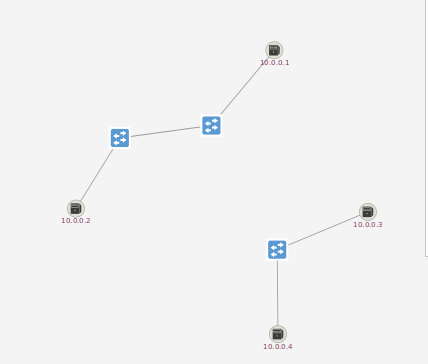
\includegraphics[width=\textwidth]{images/haikunet/error_scenario_2.png}
\caption{Initial network context in no path error}
\end{figure}

and we execute the following program:

\begin{lstlisting}[language=Ruby,breaklines=true]
source_host := Host(ip="10.0.0.2")

    destiny_host := Host(ip="10.0.0.4")

my_flow := Flow (src=source_host, dst=destiny_host, priority="55")

Intent firstExample
    Select my_flow
\end{lstlisting}

It can be seen in the image above that the error is thrown because there is no path between hosts \textit{10.0.0.2} and \textit{10.0.0.4}. 

\subsubsection{Inconsistent host definition error}

\textbf{Description:} This error is thrown when you are trying to either create or refer to a Host which already exist with different properties from the real ones. 

Let's suppose that we have the following initial network:

\begin{figure}[H]
\centering
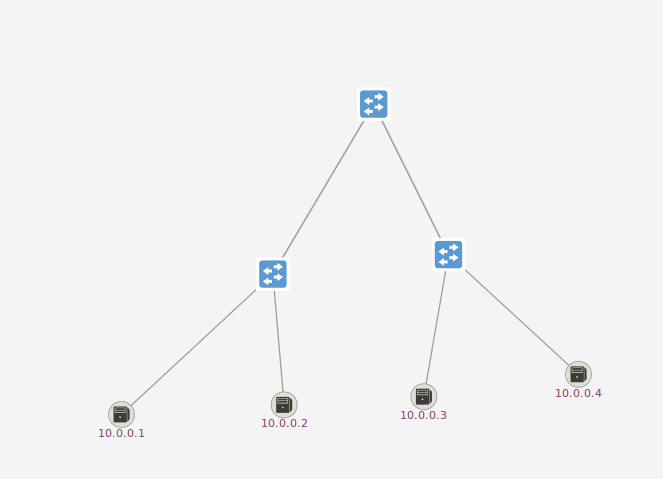
\includegraphics[width=\textwidth]{images/haikunet/error_scenario_3.png}
\caption{Initial network context in inconsistent host definition error}
\end{figure}

and we execute the following program:

\begin{lstlisting}[language=Ruby,breaklines=true]
one_host := Host(mac="9A:4A:43:D4:36:45", vlan="-1", ipAddresses=["10.0.0.1"], elementId="of:0000000000000002", port="1")

second_host := Host(mac="72:D2:0D:24:C5:36", vlan="-1", ipAddresses=["10.0.0.4"], elementId="of:0000000000000003", port="2")

my_flow := Flow (src=one_host, dst=second_host, priority="55")

Intent firstExample
    Select my_flow
\end{lstlisting}

The problem here is that we are trying to define the same host with different mac addresses. CORRECT THE IMAGE SO WE CAN SEE THE HOST WITH ITS CURRENT MAC.

\subsubsection{Percentage in loss packets error}

STILL HAS TO BE IMPLEMENTED.

\subsection{Static and Dynamic errors}

When debugging definition was made, static and dynamic errors were mentioned. We now proceed to define each type of error, and we will categorize the erros showed before in order to understand better these definitions.

\begin{itemize}

\item Static error\\
A static error can be defined as an error which can be pointed out as one, without the need of letting time pass into the underlying network. Examples of these types of erros showed before are the \textit{Flow property definition error}, \textit{No path error} and \textit{Inconsistent host definition error}
\item Dynamic error\\
A dynamic error can be defined as an erorr which needs time to be elpased in the underlying network, in order to identify it as one. An example of this kind of error is the \textit{Percentage in loss packets error}. 
\end{itemize} 

As it can be seen on the definition above, time is a variable needed for defining both kind of errors. This variable is introduced because the network is a model which is always changing, and not necesarilly just because a program changes it (for example we can always have either infraestracture or software issues, making links and host not reacheable, causing a change in the underlying network topology).\\
From the definition of both types of erros, we studied the best way to detect each of them.\\
From the first type of errors, an interpreter using a network model plus a definition of a semantic checker were implemented in order to detect them.\\ Since for detecting the second type of errors we need time to be elapsed in the underlying network, and the time needed varies depending on each error, a connection with DEVS was implemented. The key idea in this is having a representational model of the network, which can be ran as a simulation in DEVS, modelling hours of time elapsed in the network. The simulation will then replied with results, and from this results we will be able to detect if there are dynamic errors present in the program. 


\subsection{Initial Network}

The concept of initial network comes from the following view: When you apply an intent to a network, you can see the network as a mutable element which is being transformed by the application of an intent. This abstraction allow us to identify different network states that can be pointed out in the intents process: The first one, the initial one, is the network in which the user wants to apply the intent. Then there is a last one, which is the one in which the intent has already been applied, in case it was possible to do so, and is the newtork result of applying the intent. Since the intent can transform several times the network (for example first adding a host, then adding a link, etc.), we can identify all the intermediate states in which the network has to be in order to reach the last state. \\
From the given approach, in the \textbf{Future work} section we will introduce several ideas that we have related to this important concept.

\section{Language Implementation}

This section is focused to describe how each of the components detailed in the Haikunet architectural view is implemented, we will follow the processing flow as it was explained in the \textbf{Conceptual Idea} section, and start explaining how is both the lexer and parser implemented.

\subsection{Lexer/Parser}

For a better understanding of these two components, we need first to introduce the grammar of the language. 

\subsubsection{Haikunet Grammar}

The grammar of the language is as follows:

\begin{lstlisting}[breaklines=true]
Start ->	New_Network_Definition | New_Intent

New_Network_Definition ->	Identifier := Network_Elem_Def

Identifier ->	[.:A-Za-z0-9_-]+

Sring ->	[.:A-Za-z0-9_-]+

Network_Elem_Def ->	Abstract_Elem_Def | Concrete_Elem_Def

Abstract_Elem_Def ->	Action_Def | Flow_Def | Condition_Def

Concrete_Elem_Def ->	Host_Def | Link_Def | Device_Def 

Host_Def ->	Host( Params )

Link_Def ->	Link( Params )

Device_Def ->	Device( Params )

Action_Def ->	Action( Params )

Flow_Def ->	Flow( Params )

Condition_Def ->	Condition( Params )

Params -> 	Identifier = Identifier, Params | 
			Identifier = Identifier |
			Identifier = "String", Params |
			Identifier = "String" |
			Identifier = Array_Identifiers, Params |
			Identifier = Array_Identifiers 

Array_Identifiers ->	[ Elems_Of_Array ] 

Elems_Of_Array ->	Identifier  | Identifier, Elems_Of_Array

New_Intent ->				Intent Identifier
			Select Identifier	
			|    
			Intent Identifier
				Select Identifier            	
				Action Identifier                    
			| 
			Intent identifier
				Select Identifier
				Action Identifier
				Condition Identifier
\end{lstlisting}

It can be seen here that Haikunet is though for either defining the elements of the network, or defining the intent. The elements that can be defined are either concrete elements, where concrete stands up for defining elements which have a phisical representation in the network, as for example a Host, a Link and a Device, or abstract elements, where abstract represent elements as the flow, an action and a Condition. \\
For defining whatever type of element in the language, we just need to create an identifier, which will represent our element in the entire execution of the program, and define the element name in camelcase follow by the parameters needed for the creation. The nonterminal Parameters is describing to us that there is not an only way of defining an element in the language, so a question comes up which is, how should we define an element?. The answer to this question relies on the destiny of the program, and will be treated in the \textbf{Code Generation} section. \textbf{PODRÍAMOS PENSAR EN UNA FORMA DE DEFINIR CHEQUEOS SEMANTICOS DEPENDIENDO DEL DESTINY, PUES LA DEFINICIÓN DE PARAMETROS ESTA TOTALMENTE SUBEDITADA A ESTO.}

Actions and conditions are elements which are intended to be as parameters of the intent definition, and are think to work as follows:
\begin{itemize}
\item Action PENSAR MEJOR\\
An action represents a change to be done in every element that matches the identifier provided. For example, if we have the following intent definition:
\begin{lstlisting}[language=Ruby,breaklines=true]
one_host := Host(mac="9A:4A:43:D4:36:45", vlan="-1", ipAddresses=["10.0.0.1"], elementId="of:0000000000000002", port="1")

drop_packets := Action(from="9A:4A:43:D4:36:45", realize="DROP")

Intent firstExample
    Select one_host
    Action drop_packets
\end{lstlisting}

We are saying that every packet that is sent from \textit{one\_host} should be dropped. The possible actions allowed are: CUALES SON? PENSAR QUE ES LO QUE QUIERO MODELAR
\item Condition PENSAR MEJOR\\
A condition represents the act of monitoring a property in the network, and measure it in the scale detailed in the condition definition. It is always used with an action, and when the condition is satisfied, the action is performed. This is an example of use of a condition:
\begin{lstlisting}[language=Ruby,breaklines=true]
one_host := Host(mac="9A:4A:43:D4:36:45", vlan="-1", ipAddresses=["10.0.0.1"], elementId="of:0000000000000002", port="1")

one_device := Device(mac="9C:B1:C2:D4:36:12")

drop_packets := Action(from="9A:4A:43:D4:36:45", realize="DROP")

measure_of_loss_packets := Condition(one_device.packets_loss > 0.5)

Intent firstExample
    Select one_host
    Action drop_packets
    Condition measure_of_loss_packets
\end{lstlisting}
What we are doing in this case is to set an intent which describes what to do when a device starts to lose more than the 50\% of traffic. In this case, when the condition is satisfied, we start dropping packets of the host with IP \textit{10.0.0.1}.
\end{itemize}

Now that we have a better understanding of the grammar of the language, we can come back to explain in more detailed how the lexer was implemented.

\subsubsection{Lexer}

The lexer is in charge of recieving the program, and tokenize it's content. The tokens that we have identified from the grammatic presented above are the following ones: 
\begin{itemize}
\item \textbf{END\_OF\_LINE}\\
As it names points out, this token will be replaced every time the string \textit{\\n} is found
\item \textbf{EQUAL\_PARAMETERS}\\
This tokens represents the equal which is put in the paramateres definition, between parenthesis.
\item \textbf{LEFT\_PARENTHESIS}\\
This token represents the character \textit{(}
\item \textbf{RIGH\_PARENTHESIS}\\
This token represents the character \textit{)}
\item \textbf{DOUBLE\_QUOTE}\\
This token represents the character \textit{"}
\item \textbf{LFET\_BRACE}\\
This token represents the character \textit{[}
\item \textbf{RIGHT\_BRACE}\\
This token represents the character \textit{]}
\item \textbf{COMMA}\\
This token represents the character \textit{,}
\item \textbf{ASSIGN}\\
This token represents the characters \textit{:=}
\item \textbf{HOST}\\
This token represents the definition of a \textit{Host} element. The language does not take into account if the name was written in either upper case or lower case or a cambination of these.
\item \textbf{LINK}\\
This token represents the definition of a \textit{Link} element. The language does not take into account if the name was written in either upper case or lower case or a cambination of these.
\item \textbf{DEVICE}\\
This token represents the definition of a \textit{Device} element. The language does not take into account if the name was written in either upper case or lower case or a cambination of these.
\item \textbf{FLOW}\\
This token represents the definition of a \textit{Flow} element. The language does not take into account if the name was written in either upper case or lower case or a cambination of these.
\item \textbf{INTENT}\\
This token represents the definition of a \textit{Intent} element. The language does not take into account if the name was written in either upper case or lower case or a cambination of these.
\item \textbf{SELECT}\\
This token represents the definition of a \textit{Select} element. The language does not take into account if the name was written in either upper case or lower case or a cambination of these.
\item \textbf{ACTION}\\
This token represents the definition of a \textit{Action} element. The language does not take into account if the name was written in either upper case or lower case or a cambination of these.
\item \textbf{CONDITION}\\
This token represents the definition of a \textit{Condition} element. The language does not take into account if the name was written in either upper case or lower case or a cambination of these.
\end{itemize}

This lexer was implemented with the lookahead character thecnique, and can be seen as the following state machine:

\begin{figure}[H]
\centering
\includegraphics[width=\textwidth]{images/haikunet/lexer_state_diagram.png}
\caption{Lexer as a state machine}
\end{figure}

Once the lexeme is tokenize, the parser component will be in charge of detect if the program is well written. Let's see how this component was implemented.

\subsubsection{Parser}

The parser implemented for the grammatic previously described is an LL(1). Since the grammar showed before is not LL(1) friendly (since the nonterminals \textit{Params}, \textit{Elems\_of\_array} and the \textit{Initial\_simbol} make the parsing with one look ahead impossible in this context), we had to rewrite it as follows:

\begin{lstlisting}[breaklines=true]
Start -> Identifier := Network_Elem_Def     | Intent Identifier Select Identifier Intent_Prod_With_Action

Intent_Prod_With_Action ->	Action Identifier Intent_Prod_With_Condition | Lambda

Intent_Prod_With_Condition ->	Condition Identifier | Lambda

Identifier	->	[.:A-Za-z0-9_-]+

Sring	->	[.:A-Za-z0-9_-]+

Network_Elem_Def	->	Host(Params)| Link(Params)| Device(Params) | Action(Params) | Flow(Params) | Condition(Params)

Params	->	Identifier= Second_part_Equal | Lambda

Second_part_Equal	->	"String" Add_more_parameters | Identifier Add_more_parameters |  [ Elems_Of_Array ]  Add_more_parameters 

Add_more_parameters	->	,Params | Lambda

Elems_Of_Array	->	Identifier Add_more_elems_to_array | "String" Add_more_elems_to_array 

Add_more_elems_to_array	->	, Elems_Of_Array | Lambda

\end{lstlisting}

It can be easily checked that this grammar generates the same language that the one detailed before. The only new element which is present in this grammar is the \textit{Lambda} nonterminal, which represents the empty string.\\
Besides detecting programs which are not well formed, in the parser we implement the logic of constructing the abstract syntax tree, which will be used for the code generator for creating the desired output. For doing this, we extended the previous grammar to a sytax-directed translated grammar as show next:

\begin{lstlisting}[breaklines=true]
Start	->	Identifier := Network_Elem_Def  
	{
		identifiers.push(Identifier.new Identifier)
		identifiers[Identifier].val = Network_Elem_Def
	}  
|
Intent Identifier1 Select Identifier2 Intent_Prod_With_Action 
	{     
		action_and_condition = Intent_Prod_With_Action
		intents.push (Intent.new identifier1);
		intents[identifier1].select = identifier2
		intents[identifier1].action = action_and_condition['action']
		intents[identifier1].condition = action_and_condition['condition']
	}
	
Intent_Prod_With_Action	->	Action Identifier Intent_Prod_With_Condition 
		{ 
			identifier_condition = Intent_Prod_With_Condition
			return {'action':Identifier, 'condition':identifier_condition}
		}
| 
     Lambda
        {
            identifier_condition = Intent_Prod_With_Condition
            return {'action':NONE, 'condition':identifier_condition}
		}

Intent_Prod_With_Condition	->	Condition Identifier 
    {
        return Identifier
	}
| 
Lambda
    {
        return NONE
	}

Identifier	->	[.:A-Za-z0-9_-]+

Sring	->	[.:A-Za-z0-9_-]+

Network_Elem_Def	->	Host(Params)
    {
		actual_params = [ ] 
		return Host.new Params 
	}
| 
Link(Params)
    { 
    	actual_params = [ ] 
		return Link.new Params 
	}
| 
Device(Params) 
	{ 
		actual_params = [ ] 
		return Device.new Params 
	}
| 
Action(Params) 
    { 
    	actual_params = [ ] 
		return Action.new Params 
	}
|
Flow(Params)
    { 
	    actual_params = [ ] 
		return Flow.new Params 
	}
| 
Condition(Params)
    { 
	    actual_params = [ ] 
		return Condition.new Params 
	}

Params	->	Identifier= Second_part_Equal 
    { 
		actual_identifier = Identifier.new Identifier
		Second_part_Equal
	}
| 
Lambda
    {
        return actual_params
    }

Second_part_Equal	->	"String" Add_more_parameters 
    { 
        actual_identifier.val = "String"
		actual_params.push actual_identifier
		Add_more_parameters
	}
| 
Identifier Add_more_parameters 
    {
        actual_identifier.val = Identifier
		actual_params.push identifiers[actual_identifier]
		Add_more_parameters
	}
|  
[ Elems_Of_Array ]  Add_more_parameters 
{
    elems_of_array = []
    actual_identifier.val = Elems_Of_Array
	actual_params.push identifiers[actual_identifier]
	Add_more_parameters
}

Add_more_parameters	->	,Params 
    {
        Params
	}
| 
Lambda
    {
        
    }

Elems_Of_Array	->	Identifier Add_more_elems_to_array 
    { 
		elems_of_array.push identifiers[Identifier]
		Add_more_elems_to_array
 }
| 
"String" Add_more_elems_to_array 
    {
        elems_of_array.push Identifier
		Add_more_elems_to_array
    }

Add_more_elems_to_array	->	, Elems_Of_Array 
    {
        Elems_Of_Array.
	}
| 
Lambda
    {
        return elems_of_array
    }
\end{lstlisting}

Ruby is the code showed in the extended grammar above.\\
After having our program parsed, the next step is to check if the program is semantically correct. For doing this, we have implemented a semantic checker which will be explained next. 

\subsection{Semantic Checker}

The semantic checker is the component in charge of detecting static errors previously defined in the \textbf{Formal Definition} section, since we have a few quantity of these errors, we implemented the semantic checker to iterate over each of the possible errors, and try to analyze if it's present in the underlying network.\\
In this component we have as parameter both the abstract syntax tree, which was created by the parser as it was explained in the previous section, and a representation of the underlying network. For getting this representation we use the \textit{Topologygenerator}, introduced in the chapter before, as it follows: ONOS ESTA HARCODEADO, HAY QUE HACER QUE ESTO SEA PÁRAMETRICO

\begin{lstlisting}[language=Ruby,breaklines=true]
@topology_generator = Topologygenerator.new({
            "source" => "ONOS",
            "directory_concrete_builders" => "#{File.dirname(File.realpath(__FILE__))}/haikunet_builders/initial_topology_builders",
            "output_directory" => "#{ENV['HOME']}/.haikunet/initial_topology/#{@file_name}",
            "uri_resource" => uri_initial_topology 
        })
\end{lstlisting}

As you can check from the previous code, Haikunet has builders which are custom implementations focus in getting all the data which can be get from each of the elements in the network, with this we intend to make the process of detecting errors easier.

With the underlaying network representation obtained from the topologygenerator, we can now perform static checks. In case an error is found, a \textit{Semantic Error} is thrown and the execution of the program is stopped, meaning that the program never reaches it's supposed destination. You can get into more detailed in how each error checking was implemented by checking out the code. 

Now that we have our program checked, and we know that it's free of either syntactical or semantical errors, we can now proceed to generate what we have been looking out from the beginning, the desired output.

\subsection{Code Generation}

Once that we know that our program is free of the errors that we have defined, it's time to proceed to generate the output of the program. Haikunet implement's a decoupled way for doing this, which consists of dependently of the destiny recieved by argument, a class which implements the respectively code generator will be called. Adding a new code generator to Haikunet is really easy and straightforward, as you will find out in the \textbf{Implementing your CodeGenerator} tutorial in the following section.

For creating this decoupled way of associating recieving arguments with their respectively generator, Ruby modules were used. The idea of this implementation consist in the following: You select one of the destinies supported, this string is then used for include a module which has as name the argument capitalize plus the string \textit{CodeGenerator} added at the end, as it's showed in the code:

\begin{lstlisting}[language=Ruby,breaklines=true]
require_relative "#{destiny.downcase}_code_generator.rb"
self.class.send(:include, Object.const_get("#{destiny.capitalize}CodeGenerator"))
generate_output file_name
\end{lstlisting}

After including the \textit{CodeGenerator}, the function \textit{generate\_output} of the module is called. We will get into more detailed in how modules should be implemented in the \textbf{Implementing your CodeGenerator} tutorial.

Since we have three destinies supported currently, we will have for each destiny a code generator's class. The destinies are \textit{ONOS}, \textit{OPENDAYLIGHT} and \textit{DEBUG}, and their respectively code generator classes are \textit{OnosCodeGenerator}, \textit{OpenDayLightCodeGenerator} and \textit{DebugCodeGenerator}.
 The first two of them that are controllers will be explained next, and the DebugCodeGenerator class is explained in the \textbf{Debugging with DEVS} subsection which follows.

\subsubsection{Controllers}
HAY QUE TERMINAR DE IMPLEMENTAR EL OPENDAYLIGHT CODE GENERATOR!!!!.

The code to be generated, independently of the controller, will be requests to an API. What we have to do here is to define those elements which were not defined in the underlying network, eventually modified properties of one of these elements, and create and intent with their respectively logic (in case either conditions or actions are defined), for each intent defined in the program. For example, let's get into more detailed in the \textit{OnosCodeGenerator} module, in the \textit{generate\_output} function.

\begin{lstlisting}[language=Ruby,breaklines=true]
    def generate_output(file_name)
        code = ''
        requests = []
        json = ''
        @identifiers.each do |identifier|
            case identifier.value
            when HaikunetHost
                host_params = get_host_params identifier
                next if is_defined_in_topology host_params
                json = "{
                    \"mac\" : \"#{host_params['mac']}\", \n
                    \"vlan\" : \"#{host_params['vlan']}\", \n
                    \"ipAddresses\" : #{host_params['ips']}, \n
                    \"location\" : {
                        \"elementId\" : \"#{host_params['elementId']}\", \n
                        \"port\" : \"#{host_params['port']}\"
                    }
                }\n"
                requests.push({ "end_point" => "hosts", "message" => json })
                code += json
            when HaikunetFlow
                flow_params = get_flow_params identifier
                flow_params['src'].each do |src_mac|
                  flow_params['dst'].each do |dst_mac|
                    json = "{
                          \"type\": \"HostToHostIntent\",
                          \"appId\": \"org.onosproject.ovsdb\",
                          \"priority\": #{flow_params['priority']},
                          \"one\": \"#{src_mac}/-1\",
                          \"two\": \"#{dst_mac}/-1\"
                        }
                      "
                    requests.push({ "end_point" => "intents", "message" => json })
                    code += json
                  end
                end
            end
        end

        requests.each do |request|
          response = Typhoeus.post "http://127.0.0.1:8181/onos/v1/#{request['end_point']}",
                        headers: { 'Accept-Encoding' => 'application/json', 'Content-Type' => 'application/json'},
                        body: request["message"],
                        userpwd:"onos:rocks"

          raise OnosCodeGeneratorError, "When posting the following request: #{request['message']} to the endpoint #{request['end_point']}, the following error was raised #{response.body}" unless response.success?
        end

        write_file  "#{file_name[0,file_name.length-3]}_requests",
                    code
    end
\end{lstlisting}

What we are doing in this case is matching each identifier with it's corresponding json request to made to the api, for example in the \textit{HaikunetHost} identifier case, we create a JSON which has all the needed properties to create a new Host in ONOS. In the \textit{HaikunetFlow} case, what we have decided to do is to create per each \textit{(source,destiny)} pair that can be created from the flow definition, a JSON which will create a HostToHostintent. This is not the only way that we could have done this, for example, we could have either implemented a custom Intent class for our pourpose, or have used another type of intent, for example the PointToPointIntent. Our decision then was to select the HostToHostIntent, because this provided what we needed, which was to create a flow between sources and destinies, and we didn't need to implement our custom Intent, which was something that we tried to avoid, since doing this would have implied that Haikunet would have needed a custom ONOS version for running it.\\
After that every identifier which was present in the program has been translated into it's corresponding requests, what is left now it's to perform the bunch of requests recently created. In case some of this request fails, an exception is thrown describing the error, and the execution of the requests is stopped. An important thing to remark here, is that if one request fails in a bunch, then the following request after this will not be performed, but the ones before will not be undone, meaning that the network can end in an inconsistent state!. This is something that has to be done, and will be discussed later in the \textbf{Future Work} chapter.

Finally, if everything works fine, all the request will be written down in a file, just to let know the user the performed request made by the interpreter. This file can be really usefull for logging purpouses.

\subsubsection{DebugCodeGenerator}

This is the code generator which will be called in case \textit{DEBUG} option is received as argument. In this subsection we want to introduce the model which will be used to simulate the network, the default parameters that will be set, how is the communication between the simulator and the interpreter, and explain how should this option be used.

Let's first understand what is the \textit{DebugCodeGenerator} purpose. As it was explained in the \textbf{Formal Definition} section, debugging here means finding errors before the intent is applied to the network, in order to detect some kind of errors, for example dynamic ones, instead of applying directly the program to a functional network and find out which are the errors introduced, we give the user another way, the simulation way. What does it mean?, that when the \textit{DEBUG} option is selected, the model of the underlying network will be converted to a simulation model, the program will be applied to this model, and finally the model will be ran in DEVS. After the running, results will be showed to the user, and from these results we would be able to check if the network behaves as expected. This is the \textit{DebugCodeGenerator} purpose, to give the user the ability of testing Haikunet program's without affecting an operational network.\\
Now that we understand the purpose, let's understand how do we translate a program:

CONTINUAR

\section{Tutorial}

\subsection{Installation}

\textbf{Pre-requisite:} You need to have a git client installed, a machine running a Linux distribution (it was tested in an Ubuntus machine, but should work in any Linux distribution machine), and already installed a ruby version equal or major to 2.0.0.

For installing Haikunet, just run the following commands:

\begin{lstlisting}[language=bash,breaklines=true]
$ git clone git@github.com:andyLaurito92/haikunet.git
$ cd haikunet
$ sudo ./install_haikunet.sh 
\end{lstlisting}

And that's it!, you have already installed the interpreter. Let's understand a bit more about the language before jumping into the code.

\subsection{Using the interpreter}

\textbf{Pre-requisite:} Have running locally the ONOS controller, and have already download the language repository.

For running the Haikunet interpreter, you will need: 
\begin{itemize}
\item The path to the file where the haikunet program is (remember that only files with the ".hk" extension are allowed).
\item Specify one of the destinations supported (the current supported are \textit{ONOS}, \textit{OPENDAYLIGHT} and \textit{DEBUG}).
\item An URI from where to obtain the initial topology.
\end{itemize}

Let's get into more detailed in the last two arguments.\\
The destination argument is an option which will tell the interpreter to which destiny has to generate the code of the input program, the options current supported are \textit{ONOS}, \textit{OPENDAYLIGHT} and \textit{DEBUG}. The first two are controllers, and selecting one of them will generate a bunch of request to the corresponding API REST. The DEBUG option will generate a simulation in DEVS, taking as initial topology the one specified by argument, and will show you simulations result's once the run is complete. The idea is that with this results, you will be able to identify if the network behaviour is the one you expected. We will get into more detailed on this in the \textbf{Implementing your first program} subsection.\\
The other argument is the URI from the Initial Network, which was already explained in the \textbf{Formal Definition} section. As the name remarks, will be either a URI of an API REST of a controller, or a path to a file which will contain a ruby NTM (this was explained in the previous chapter, in the \textbf{Network Topology Model} section).\\

Let's now suppose that:
\begin{itemize}
\item We want to execute the \textit{host\_to\_host.hk} program (you can find it in \textit{\$HAIKUNET\_DIRECTORY/examples/programs}), which creates two host if they don't exist in the underlying network, and creates a flow between them. 
\item We are using ONOS as destiny output.
\item We will use as initial topology the one that we have at ONOS. 
\end{itemize} 

This is how you use the interpreter for doing that (we will assume that you will execute the haikunet interpreter from the \textit{\$HAIKUNET\_DIRECTORY}, and the ONOS local version that you are running can be located at http://127.0.0.1:8181 address):

\begin{lstlisting}[language=bash,breaklines=true]
$ haikunet program -n examples/programs/host_to_host.hk -d ONOS -u http://127.0.0.1:8181/onos/v1/
\end{lstlisting}

In the previous command:
\begin{itemize}
\item \textbf{-n} is the option to provide the path to the interpreter.
\item \textbf{-d} is the destiny name.
\item \textbf{-u} is the path to the uri initial topology.
\end{itemize}

If you want to debug the same program using the same initial topology, just run the following command:

\begin{lstlisting}[language=bash,breaklines=true]
$ haikunet program -n examples/programs/host_to_host.hk -d DEBUG -u http://127.0.0.1:8181/onos/v1/
\end{lstlisting}

You may also want to try to use as initial topology the one provided in \textit{examples/initial\_topologies} to debug it. The command to run in this case is:

\begin{lstlisting}[language=bash,breaklines=true]
$ haikunet program -n examples/programs/host_to_host.hk -d DEBUG -u examples/initial_topologies/example_topology.rb
\end{lstlisting}

In case your default controller is OpenDayLight, you just have to use the OPENDAYLIGHT destiny, and specify the uri \textit{http://OPEN\_DAY\_LIGHT\_IP:8080/restconf/operational/network-topology:network-topology/topology/flow:1/}, where \textit{OPEN\_DAY\_LIGHT\_IP} stands for the corresponding IP address of the controller. 

You can find these and more examples in the interpreter help's by running the following command:

\begin{lstlisting}[language=bash,breaklines=true]
$ haikunet program --help
\end{lstlisting}

Now that we know how to use the interpreter, let's write our first program!.

\subsection{Implementing your first program}

\subsection{Implementing your CodeGenerator}

\section{Future work}